\chapter{Background}
\label{chap:background}

This chapter provides some background knowledge that will be useful in
understanding the work presented in this thesis.
Section~\ref{sec:background.rts} discusses some terminology related to
real-time systems that will be used throughout the thesis.
Section~\ref{sec:background.monitoring} describes run-time monitoring
techniques for security and reliability which will be used in
Chapters~\ref{chap:monitoring_wcet}, \ref{chap:monitoring_hard_drop}, and
\ref{chap:monitoring_dift_drop}.

\section{Real-Time Systems}
\label{sec:background.rts}

% Tasks and jobs
\begin{figure}
  \begin{center}
    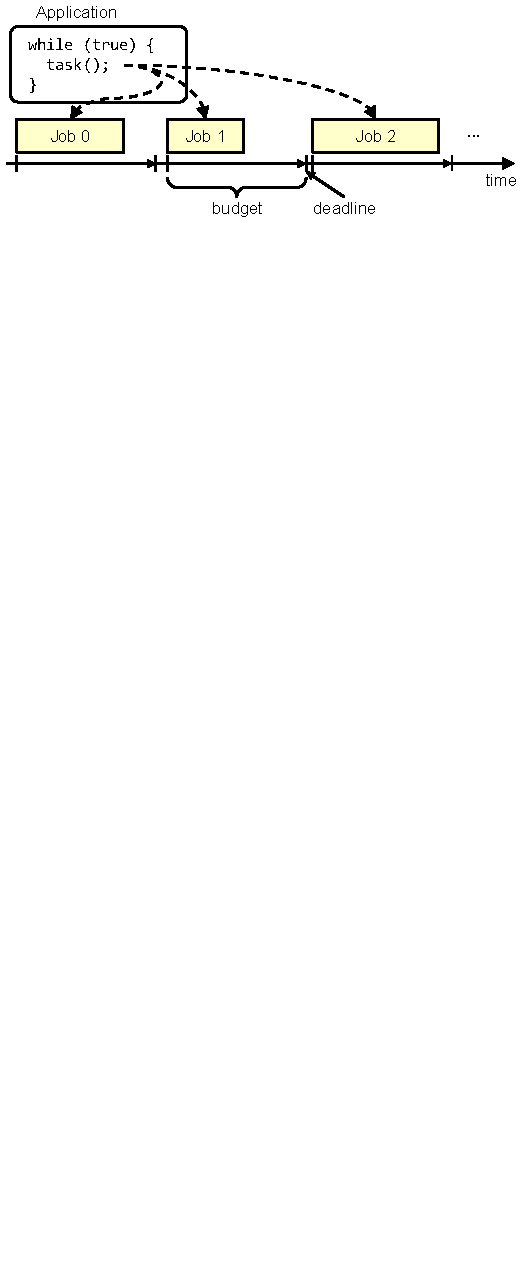
\includegraphics{exec_time_prediction/figs/jobs.pdf}
    \caption{Example of tasks, jobs, and deadlines.}
    \label{fig:exec_time_prediction.applications.jobs}
  \end{center}
\end{figure}

A real-time system application is typically specified as a set of \emph{tasks}
which have timing requirements. We refer to the time period in which a task
must complete as its \emph{time budget}. For example, games are typically
written with a main task that handles reading user input, updating game state,
and displaying the output. In order to maintain a certain frame rate (e.g., 30
frames per second), this task must finish within the frame period budget (e.g.,
33 milliseconds for 30 frames per second operation).

We define a \emph{job} as a dynamic instance of a task.
Figure~\ref{fig:exec_time_prediction.applications.jobs} shows how a task maps
to multiple jobs. Each job has a \emph{deadline} which is the time by which it must
finish execution. For example, for a game running at 30 frames-per-second, 30
jobs for the game loop task are run each second. Each of these jobs has a
deadline which is 33 milliseconds after the job's start time. These jobs all
correspond to the same set of static task code, but their dynamic behavior
differs due to different inputs and program state. For example, one job may see
that the user has pressed a button and thus execute code to process this button
press. Other jobs may see no new user input and skip the need to process user
input.  As a result, job execution times can vary depending on input and
program state.

% Timings (WCET, actual exec time, etc.)
\begin{figure}
  \begin{center}
    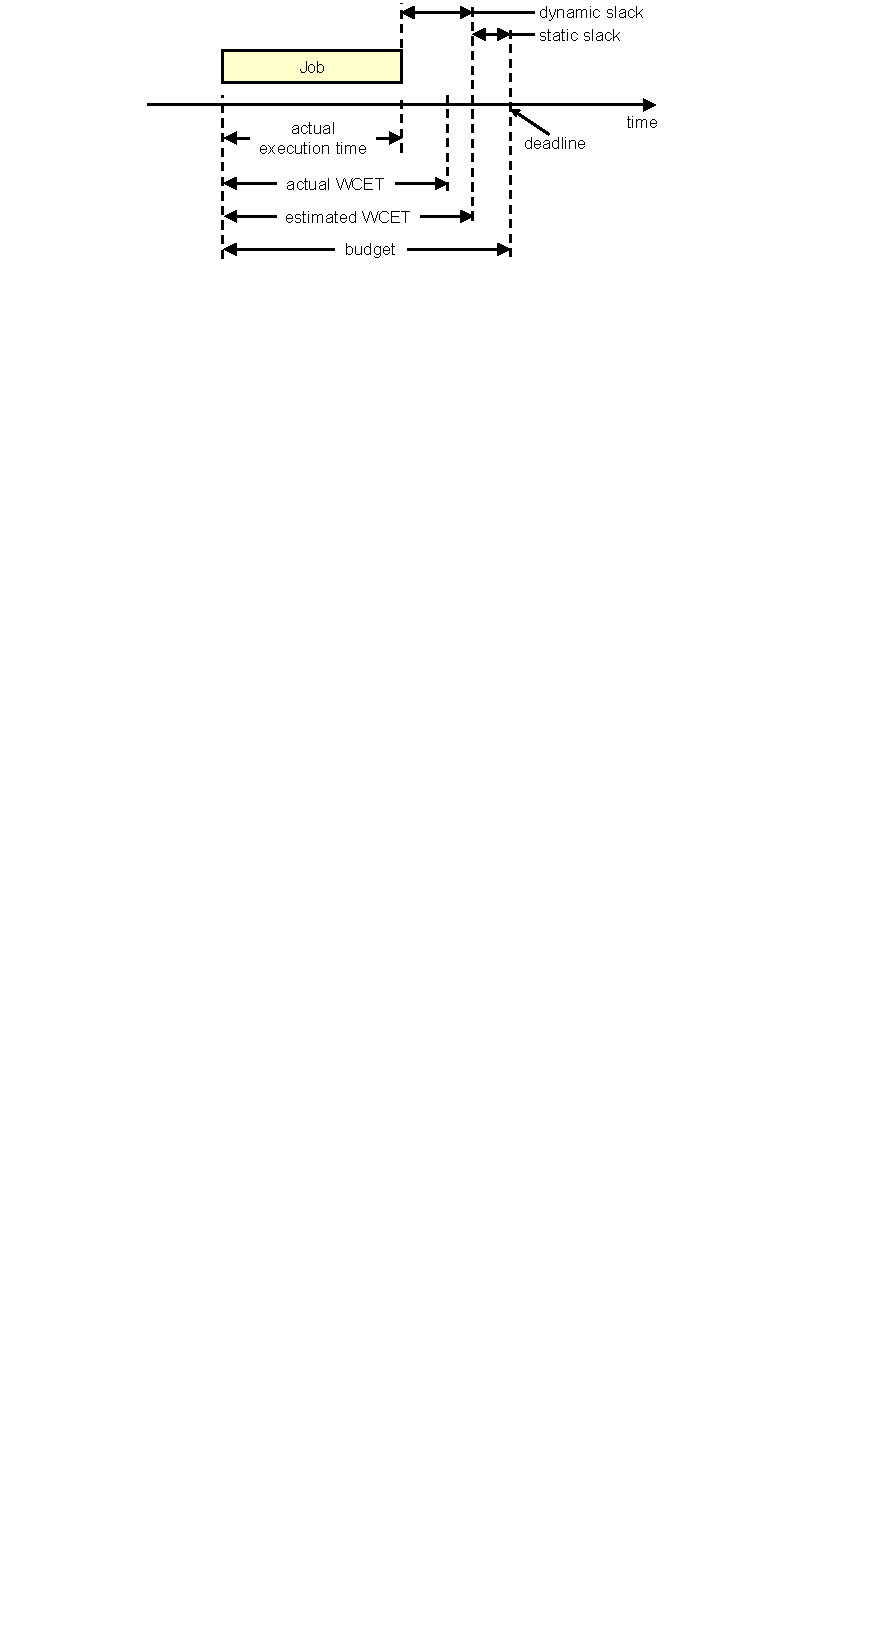
\includegraphics{figs/timings.pdf}
    \caption{Timings related to a job.}
    \label{fig:background.rts.timings}
  \end{center}
\end{figure}

There are several times of interest for a job when dealing with real-time
systems (see Figure~\ref{fig:background.rts.timings}). The time that it takes a
job to finish is its \emph{actual execution time}. The worst-case execution
time of the task across all possible inputs and initial states is its
\emph{actual worst-case execution time (WCET)}. Tasks are statically analyzed
to produce an \emph{estimated worst-case execution time (WCET)} for timing
analysis and scheduling. This estimated WCET is guaranteed to be conservative
(i.e., it is greater than or equal to the actual WCET).  The time between the
estimated WCET and the deadline is the \emph{static slack} that exists. That
is, the schedule could be adjusted to reduce the deadline and still guarantee
that tasks finish on time. On the other hand, we refer to the difference in
actual execution time and estimated WCET as the \emph{dynamic slack}. This is
the slack time that is only available at run-time.

\section{Run-Time Monitoring}
\label{sec:background.monitoring}

\subsection{Architecture Overview}

% Parallel programmable monitoring
There are several options on how to implement run-time monitoring.
Implementing run-time monitoring in software using binary instrumentation or
other similar methods introduces especially high overheads. For example,
dynamic information flow tracking (DIFT) implemented in software suffers a 3.6x
slowdown on average \cite{qin06-lift}. Implementing monitors in hardware
greatly decreases the performance impact by performing monitoring in parallel
to a program's execution. A dedicated hardware implementation of DIFT reduces
average performance overheads to just 1.1\% \cite{suh-dift-asplos04}.  However,
fixed hardware loses the programmability of software. A fixed hardware
implementation cannot be updated and cannot change the type of run-time
monitoring performed. Thus, recent studies have proposed using programmable
parallel hardware, such as extra cores in a multi-core system or FPGA
coprocessors, for monitoring \cite{chen08-lba, flexcore-micro10,
harmoni-dsn12}. Our work in this thesis is targeted at these programmable
parallel hardware monitors.

% Monitoring architecture
\begin{figure}
  \begin{center}
    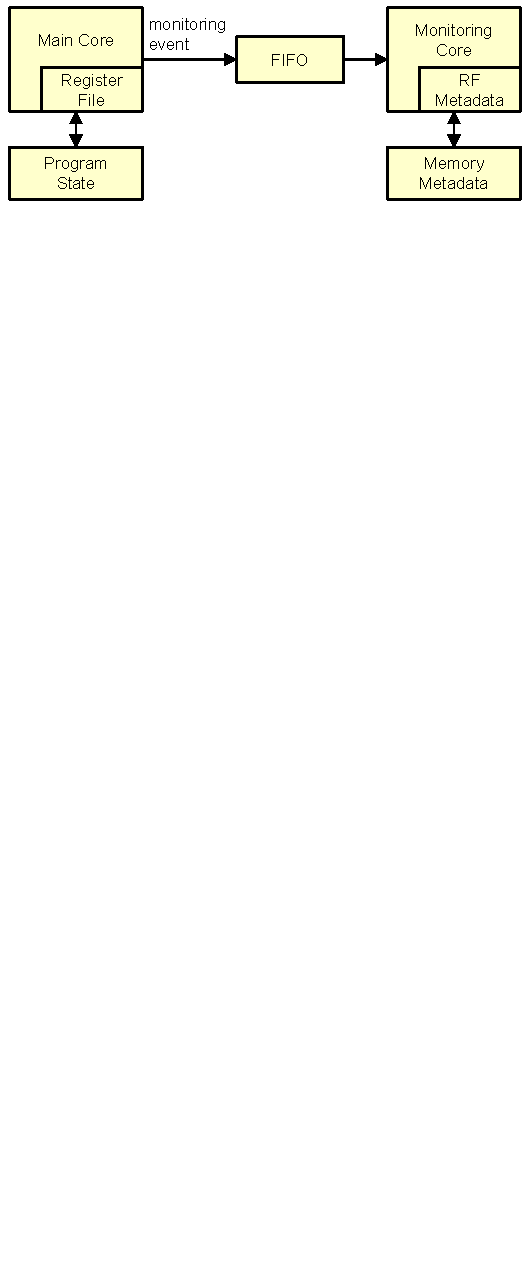
\includegraphics[width=3.5in]{monitoring_wcet/figs/arch.pdf}
    \caption{Parallel monitoring architecture model.}
    \label{fig:monitoring_wcet.monitoring.arch} 
  \end{center}
\end{figure}

% Automatically forward instructions
\begin{figure}
  \begin{center}
    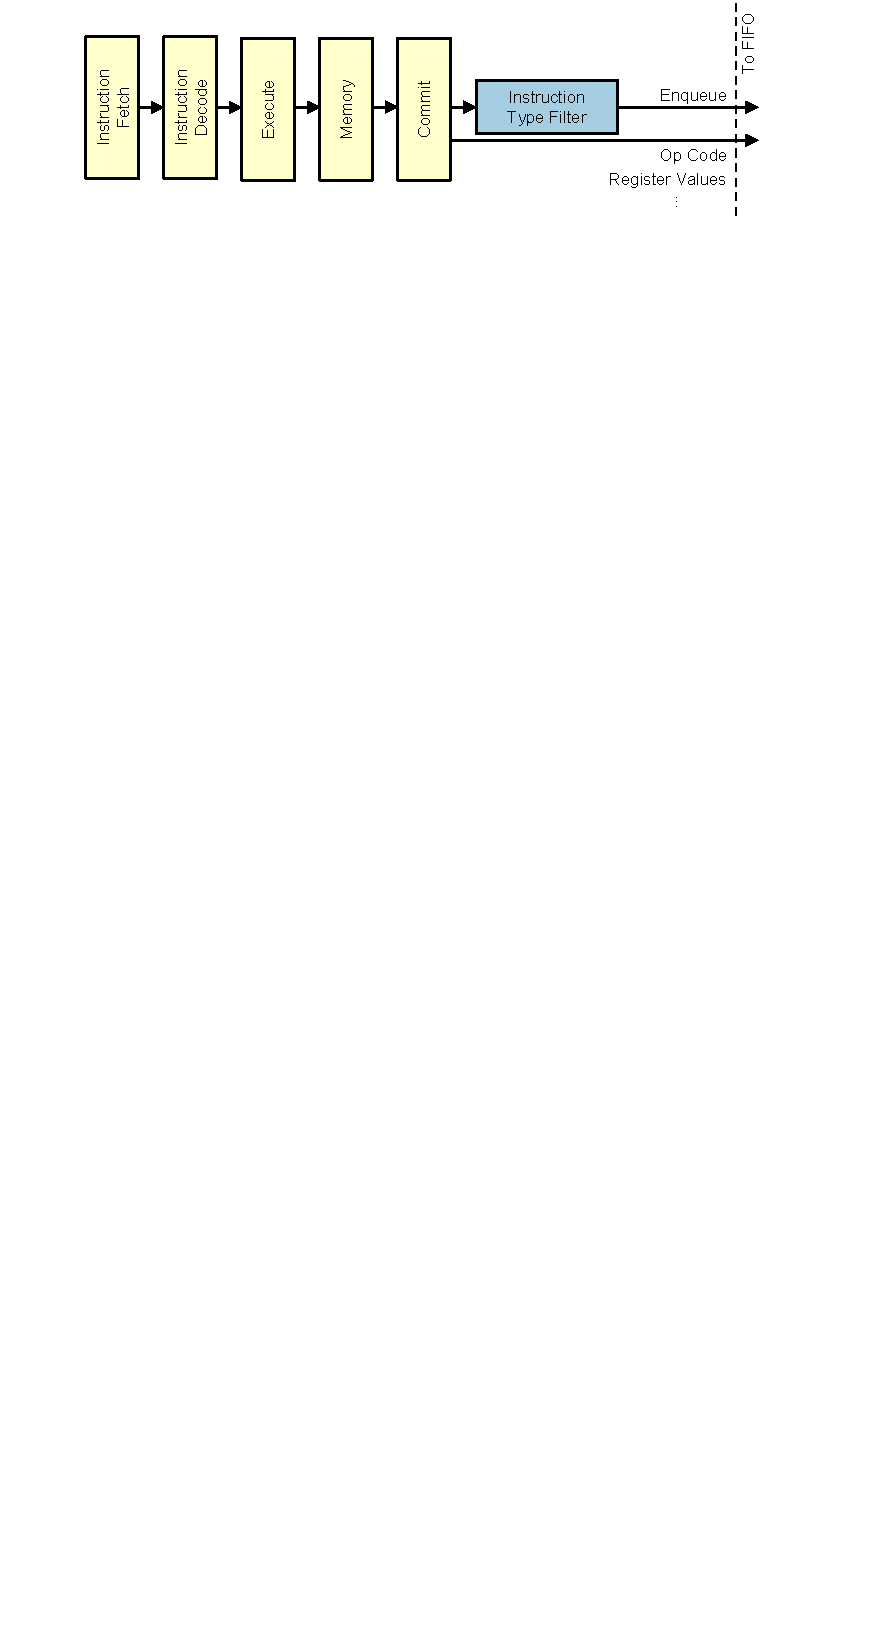
\includegraphics{monitoring_wcet/figs/forwarding.pdf}
    \caption{The main core pipeline is modified to forward information on certain
    instruction types.}
    \label{fig:monitoring_wcet.monitoring.forwarding}
  \end{center}
\end{figure}

Figure~\ref{fig:monitoring_wcet.monitoring.arch} shows a model of the
run-time parallel monitoring architecture that is assumed in this thesis. The
architecture consists of two parallel processing elements, main and monitoring
cores, which are loosely coupled with a FIFO buffer.  The main core runs a
computation task, called the {\em main task}, which performs the original
function of the real-time system.  The monitoring core receives a trace of
certain main task instructions through a FIFO, and performs a {\em monitoring
task} in parallel in order to check whether the system is operating properly.
We refer to the main task instructions that need to be sent to the monitoring
core as {\em forwarded instructions} or {\em monitored instructions}. The
forwarded instructions are determined based on a particular monitoring
technique, and are sent by the main core transparently without explicit
instructions added to the main task.
Figure~\ref{fig:monitoring_wcet.monitoring.forwarding} shows how an example
main core pipeline can be modified to automatically forward information when
instructions of certain types are committed. When an instruction commits, a
comparator checks whether the opcode of the committed instruction is one that
should be forwarded. If the instruction should be forwarded, then an enqueue
signal is sent to the FIFO.  Information about the instruction that is needed
for monitoring, such as register values, memory locations accessed, etc., is
stored in the FIFO. In this way, the detection and handling of monitoring
events is handled in hardware, with no need to modify the main task.

The forwarded instruction triggers the monitoring core to execute a series of
monitoring instructions.  A different monitoring task is executed depending on
the type of forwarded instruction. We refer to the collection of monitoring
tasks as a \emph{monitor} or a \emph{monitoring scheme}. Different monitoring
schemes seek to ensure different run-time properties.  Monitors typically
maintain metadata corresponding to each memory location ({\tt
mem\_metadata[addr]}) and register ({\tt rf\_metadata[reg\_id]}) of the main
core.  If the monitoring scheme detects an inconsistent or undesired behavior
in the sequence of monitoring events, then an error is detected. We do not
focus here on how to handle such an error. However, there are several options
on how to handle such an error such as raising an exception, notifying the
user, or switching to a simple, more trusted main task \cite{sha-simplex-sw01}.

% Pipeline diagram to show stalls
\begin{figure}
  \begin{center}
    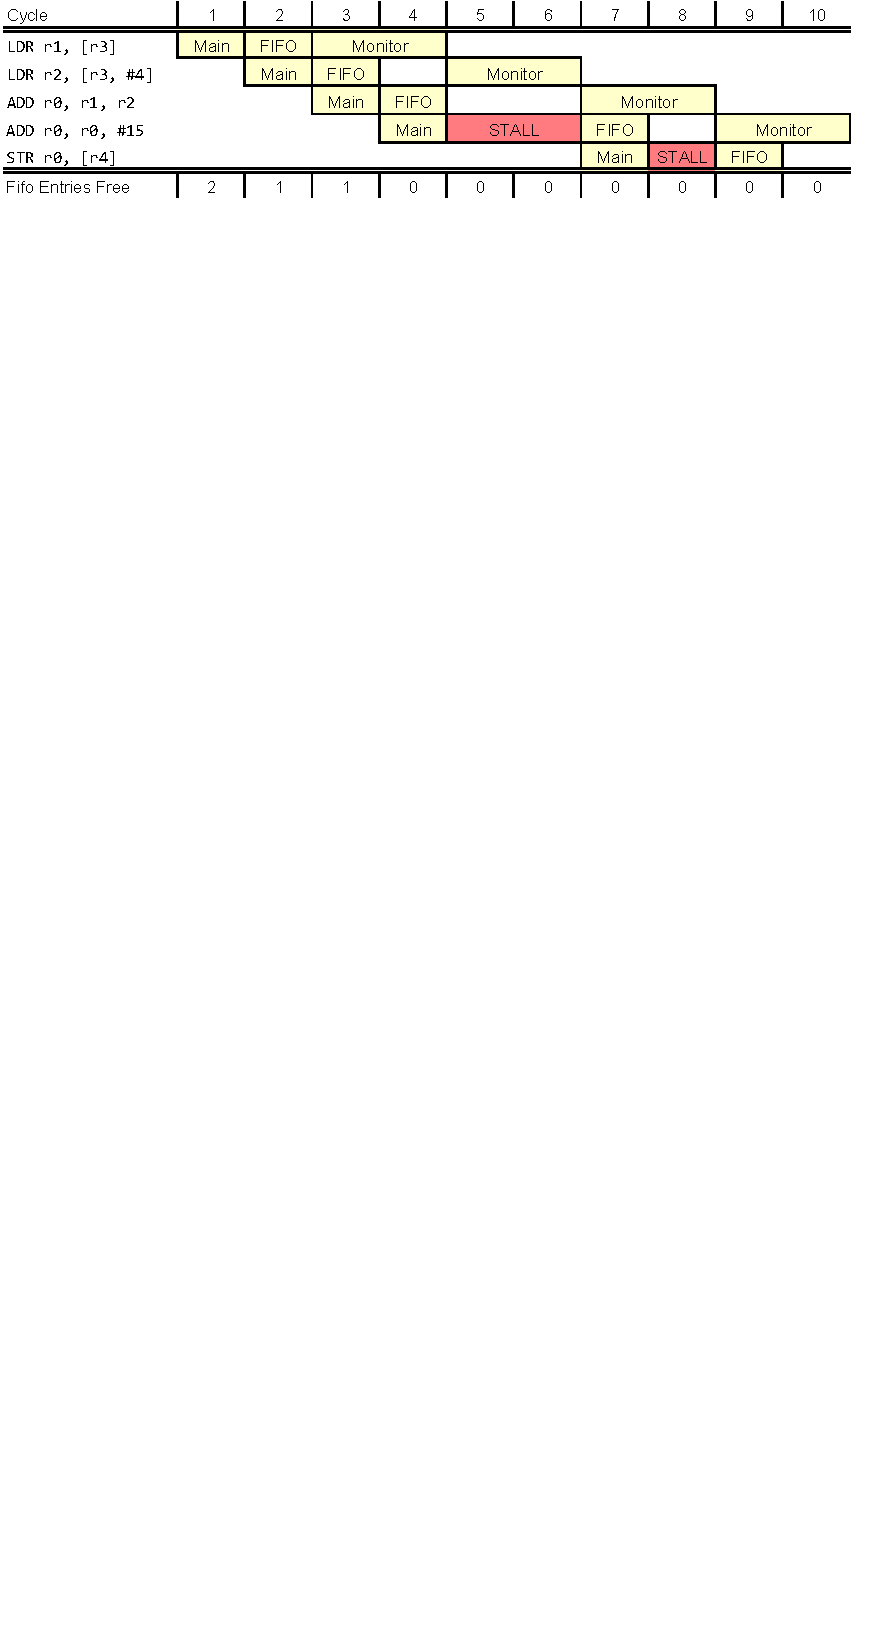
\includegraphics{monitoring_wcet/figs/pipeline.pdf}
    \caption{Pipeline diagram of monitoring. The main core stalls due to the
    slower throughput of the monitor.}
    \label{fig:monitoring_wcet.monitoring.pipeline}
  \end{center}
\end{figure}

In order to decouple the execution of the main task and the monitoring task, a
dedicated hardware FIFO is used to buffer monitoring events between the main
core and the monitoring core.  In the ideal case, the monitoring task operates
in parallel with the main task.  However, since 
every forwarded instruction of the main task
takes several instructions to monitor, the monitoring core is not always able to keep
up with the throughput of monitoring events generated by the main core.  Thus,
when the FIFO is full, the main core is forced to stall on monitoring events.
Figure~\ref{fig:monitoring_wcet.monitoring.pipeline} shows an example
execution where a series of instructions are monitored. In this simple example,
the FIFO only has 2 entries and it takes the monitoring task 2 cycles to
process a monitoring event. For simplicity, only the commit stage of the main
core pipeline is shown.  After the 4th instruction ({\tt ADD}) is committed by
the main core, the FIFO is full and the monitoring core is busy. Thus, in order
to not miss information about a monitoring event, the main core must stall
before continuing execution and committing the 5th instruction ({\tt STR}).
These stalls due to the mismatch in throughput are a major source of overhead.
We refer to these stalls of the main core due to monitoring as \emph{monitoring
stalls} and the number of cycles stalled as \emph{monitoring stall cycles}. In
the example code sequence shown, three monitoring stall cycles occur, two for
instruction 4 and one for instruction 5.

\subsection{Example Monitoring Scheme}
\label{sec:monitoring_wcet.monitoring.example}

There are many possible monitoring schemes that can be implemented on this type
of fine-grained parallel monitoring architecture such as memory protection
\cite{mondrian-asplos02}, information flow tracking \cite{dift-asplos04,
testudo-micro08}, control flow integrity checking \cite{hafix-dac15}, soft error
detection \cite{argus-micro07}, data-race
detection \cite{cord-hpca06, eraser-tocs97, literace-pldi09, pacer-pldi10},
etc.  For example, an array bounds check (BC) \cite{hardbound-asplos08} can be
implemented in order to detect when software attempts to read or write to a
memory location outside of an array's bounds. This can be done by associating
metadata with array pointers that indicate the arrays' base (start) and bound
(end) addresses. On loads or stores with the array pointer, the monitor checks
that the memory address accessed is within the base and bound addresses. In
addition, this base and bound metadata is propagated on ALU and memory
instructions to track the corresponding array pointers.

% Example monitor (BC)
\begin{figure}
  \begin{center}
    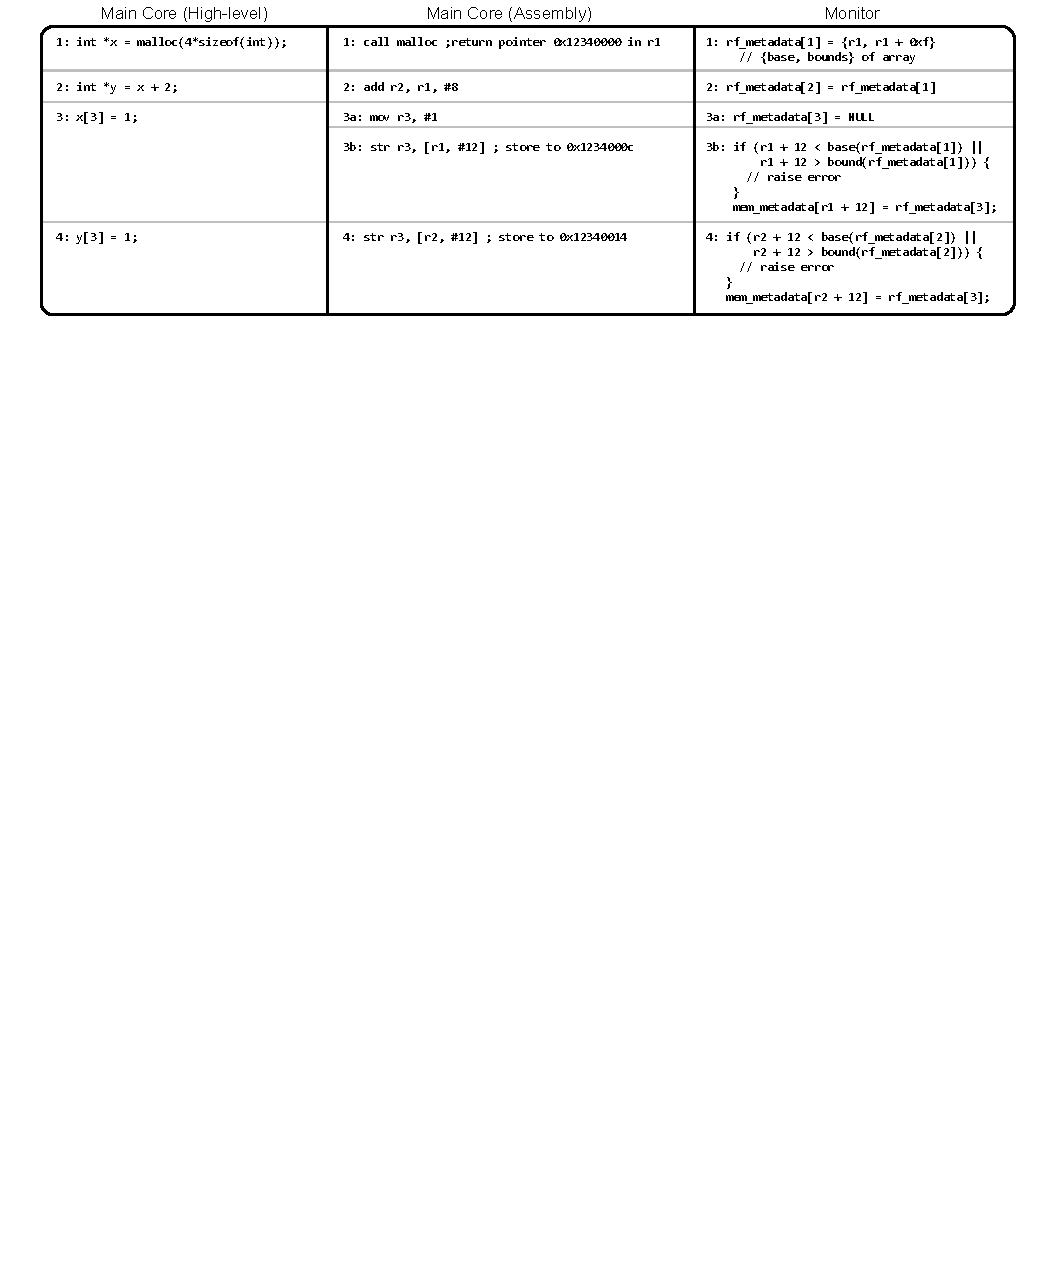
\includegraphics{monitoring_wcet/figs/example_full.pdf}
    \caption{Example of array bounds check monitor.}
    \label{fig:monitoring_wcet.monitoring.example_full}
  \end{center}
\end{figure} 

Figure~\ref{fig:monitoring_wcet.monitoring.example_full} shows an example
pseudo-code segment, its assembly level instructions, and the corresponding
monitoring operations for an array bounds check monitor.  First, an array {\tt
x} is allocated using {\tt malloc} (line 1).  As {\tt malloc} returns the
array's address in a register, the monitor associates base and bounds metadata
with the corresponding register.  Next, pointer {\tt y} is set to point to the
middle of array {\tt x} (line 2).  At the assembly level, a register {\tt r2}
is set to array {\tt x}'s address plus an offset.  The monitor propagates the
metadata of the original pointer in {\tt r1} to the metadata of {\tt r2}. This
is to ensure that pointer {\tt y} is not used to exceed the array's bounds.
Line 3a shows setting register {\tt r3} to a constant value of 1.  When this
happens, {\tt r3}'s metadata is reset to NULL in case it previously stored a
pointer.  Finally, the value of {\tt r3} is written to memory using both
pointers {\tt x} and {\tt y}.  In both cases, the monitor checks whether the
store address is within the bounds of the register metadata. In the first case
(line 3b), {\tt x+12} is within the original array's bounds. No error is raised
and the metadata of {\tt r3} is propagated to the metadata of the store
address. If {\tt r3} were a pointer, then this would allow a future instruction
to load the pointer and use it to access its corresponding array or data
structure. In the second case, {\tt y+12} (line 4) corresponds to {\tt x+20}
which is not within the array's bounds and the monitor will raise an error. 

Note that this monitoring is performed automatically and transparently with
almost no modification needed to the main program. The only modification to the
main program that is needed is to initially set metadata, such as setting the
base and bounds addresses on a {\tt malloc} call for array bounds checking.
The propagation and checks of the metadata occur automatically as instructions
are forwarded to the monitor.  Here, we have shown the dynamic sequence of
operations executed by the monitor, but the actual static code consists of a
set of instructions to be run for each possible instruction type (load, store,
etc.). Only instruction types relevant for the particular monitoring scheme are
forwarded.



